\documentclass[aspectratio=169]{beamer}

\usepackage[T1]{fontenc}
\usepackage{graphicx}
\usepackage{tikz}
\usepackage{booktabs}
\usepackage{minted}
\usepackage{hyperref}
\usepackage[dvipsnames]{xcolor}
\usepackage[spanish]{babel}

\usetikzlibrary{shapes.geometric, arrows.meta, positioning}
\tikzstyle{startstop} = [rectangle, rounded corners, minimum width=3cm, minimum height=1cm,text centered, draw=black, fill=blue!20]
\tikzstyle{process} = [rectangle, minimum width=3.2cm, minimum height=1cm, text centered, draw=black, fill=gray!10]
\tikzstyle{io} = [trapezium, trapezium left angle=70, trapezium right angle=110, minimum width=3.2cm, minimum height=1cm, text centered, draw=black, fill=orange!20]
\tikzstyle{arrow} = [thick, ->, >=stealth]
\usemintedstyle{manni}

\usetheme{Berlin}
\setbeamercolor{structure}{fg=RoyalPurple}
\setbeamertemplate{headline}{}
\setbeamertemplate{navigation symbols}{}
\makeatletter
\setbeamertemplate{footline}{
  \ifnum\insertframenumber>2
    \leavevmode%
    \hbox{%
      \begin{beamercolorbox}[wd=0.5\paperwidth,ht=2.5ex,dp=1ex,center]{title in head/foot}%
        \usebeamerfont{title in head/foot}\insertsection
      \end{beamercolorbox}%
      \begin{beamercolorbox}[wd=0.5\paperwidth,ht=2.5ex,dp=1ex,right]{page number in head/foot}%
        \usebeamerfont{page number in head/foot}\insertframenumber{} / \inserttotalframenumber\hspace{1em}
      \end{beamercolorbox}%
    }%
    \vskip0pt%
  \fi
}
\makeatother

\title[Motor y editor de videojuegos en 2D enfocado al desarrollo de juegos RPG]{Motor y editor de videojuegos en 2D enfocado al desarrollo de juegos RPG}
\subtitle{2D video game engine and editor focused on RPG game development}
\author[Miguel Curros, Alejandro González y Alejandro Massó]{Miguel Curros García\\ Alejandro González Sánchez\\ Alejandro Massó Martínez}
\date{10 de junio de 2025}

\newcommand{\baker}{%
	\textsc{RPGBaker}%
}

\newcommand{\comillas}[1]{\guillemotleft #1\guillemotright{}}

\begin{document}

\frame{\titlepage}

\begin{frame}{Índice}
	\tableofcontents
\end{frame}

\section{Objetivos}
\begin{frame}{Objetivos}
	\begin{columns}
		\column{0.7\textwidth}
		\begin{itemize}
			\item Motor 2D multiplataforma orientado a RPG.
			\item Juegos definidos en archivos de datos.
			\item Editor que permita diseñar los juegos.
		\end{itemize}
		\column{0.3\textwidth}
		
\includegraphics[width=0.8\textwidth]{imgs/objetivos/android.pdf}
	\end{columns}
\end{frame}

\section{Herramientas}
\begin{frame}{Herramientas}
	\begin{columns}
		\column{0.5\textwidth}
		\begin{itemize}
			\item Desarrollo en C++.
			\item Motor con SDL.
			\item Archivos de datos en Lua.
			\item Editor con SDL y DearImGui.
		\end{itemize}
		\column{0.5\textwidth}
		\begin{center}
			
\includegraphics[width=0.6\textwidth]{imgs/herramientas/sdl.pdf}
			\begin{columns}
				\column{0.4\textwidth}
				
\includegraphics[width=\textwidth]{imgs/herramientas/lua.pdf}
				\column{0.6\textwidth}
				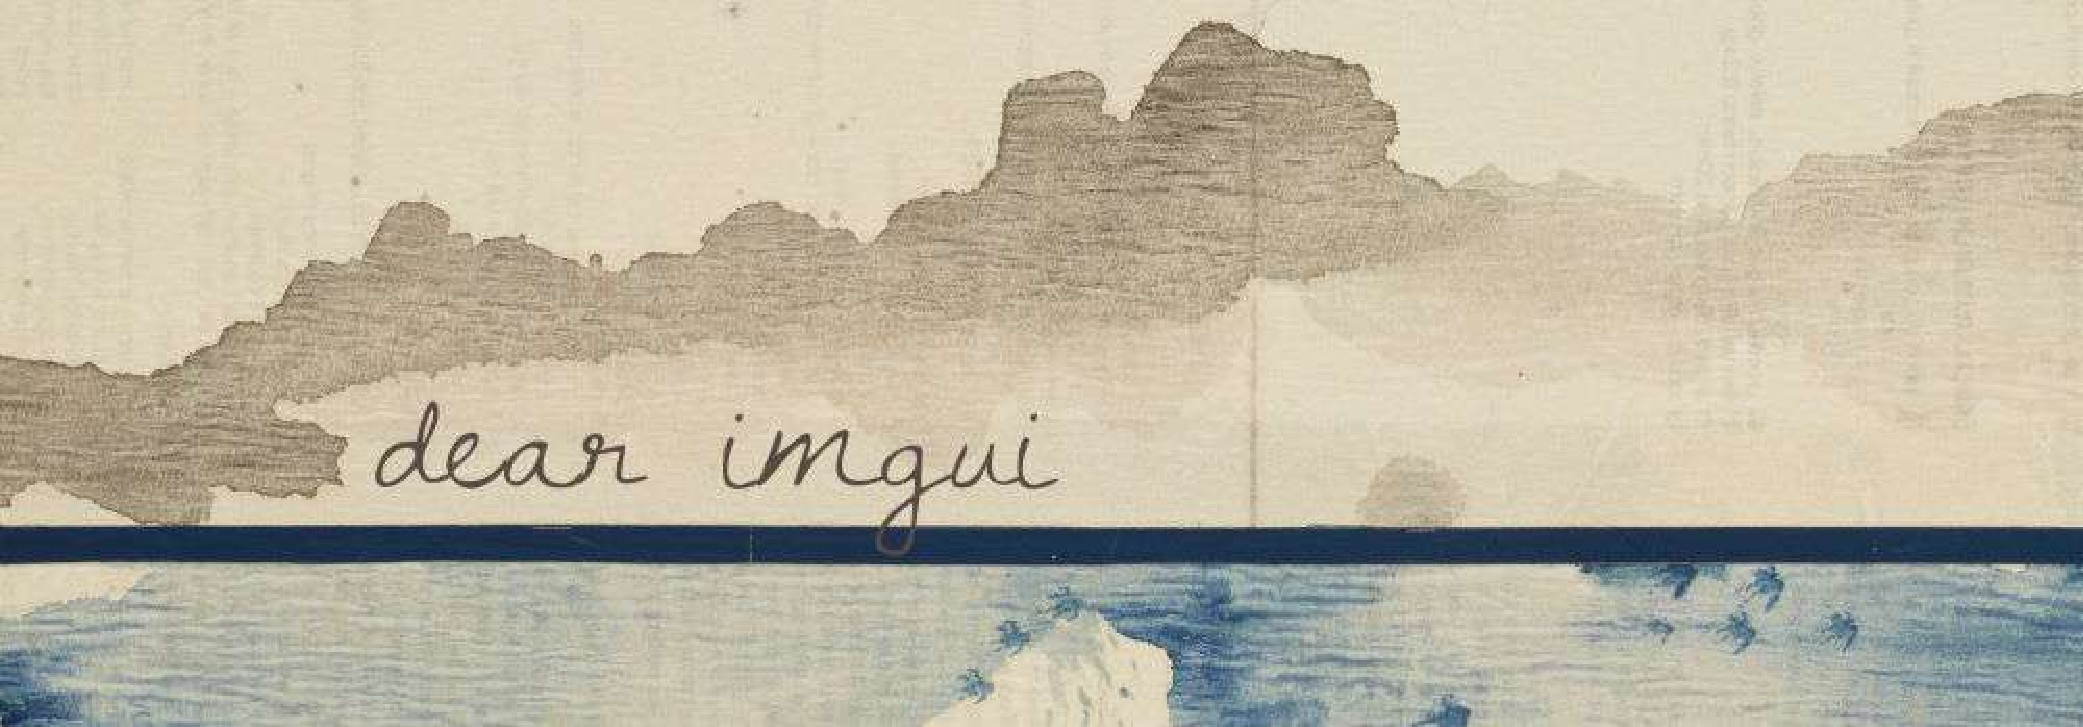
\includegraphics[width=\textwidth]{imgs/herramientas/dearimgui.pdf}
			\end{columns}
		\end{center}
	\end{columns}
\end{frame}
\section{Diseño del motor de \baker}
\begin{frame}{\textit{Core}}
	\begin{columns}
		\column{0.5\textwidth}
			\begin{itemize}
				\item Sistema de entidad componente.
				\item Sistema de recursos.
			\end{itemize}
		\column{0.5\textwidth}	
			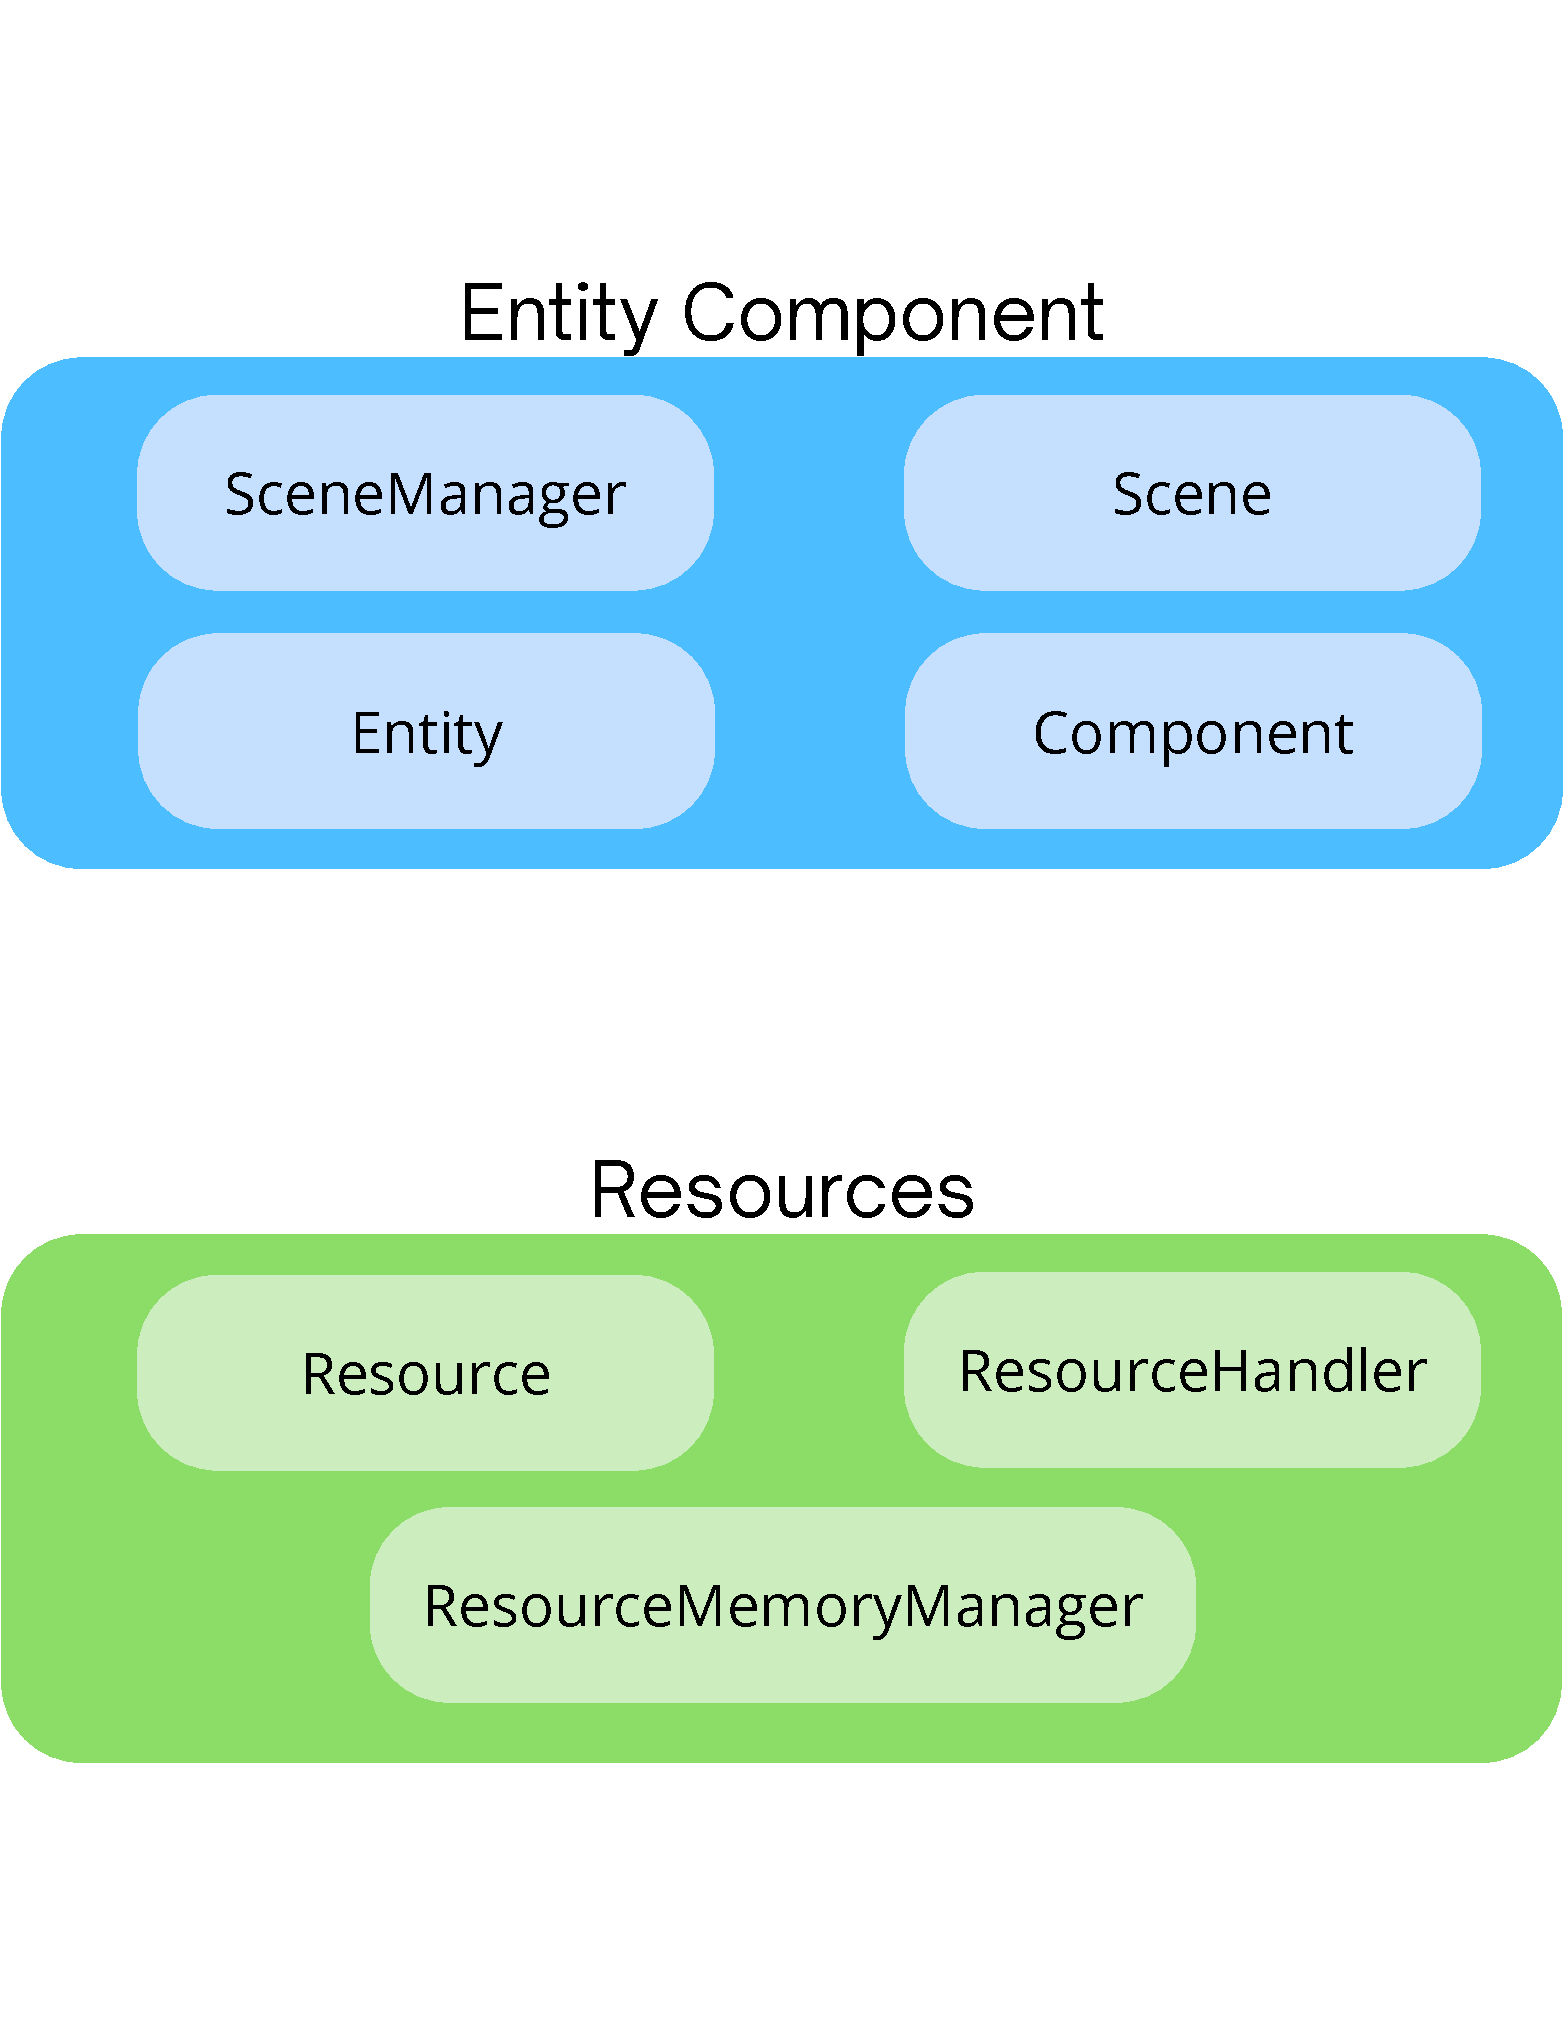
\includegraphics[height=0.85\textheight]{imgs/motor/Core.pdf}
	\end{columns}
\end{frame}
\begin{frame}{Componentes genéricos}
	\begin{columns}
		\column{0.5\textwidth}
		\begin{itemize}
			\item Sistema de \textit{renderizado}.
			\item Sistema de audio.
			\item Sistema de \textit{input}.
			\item Sistema de colisiones.
		\end{itemize}
		\column{0.5\textwidth}
			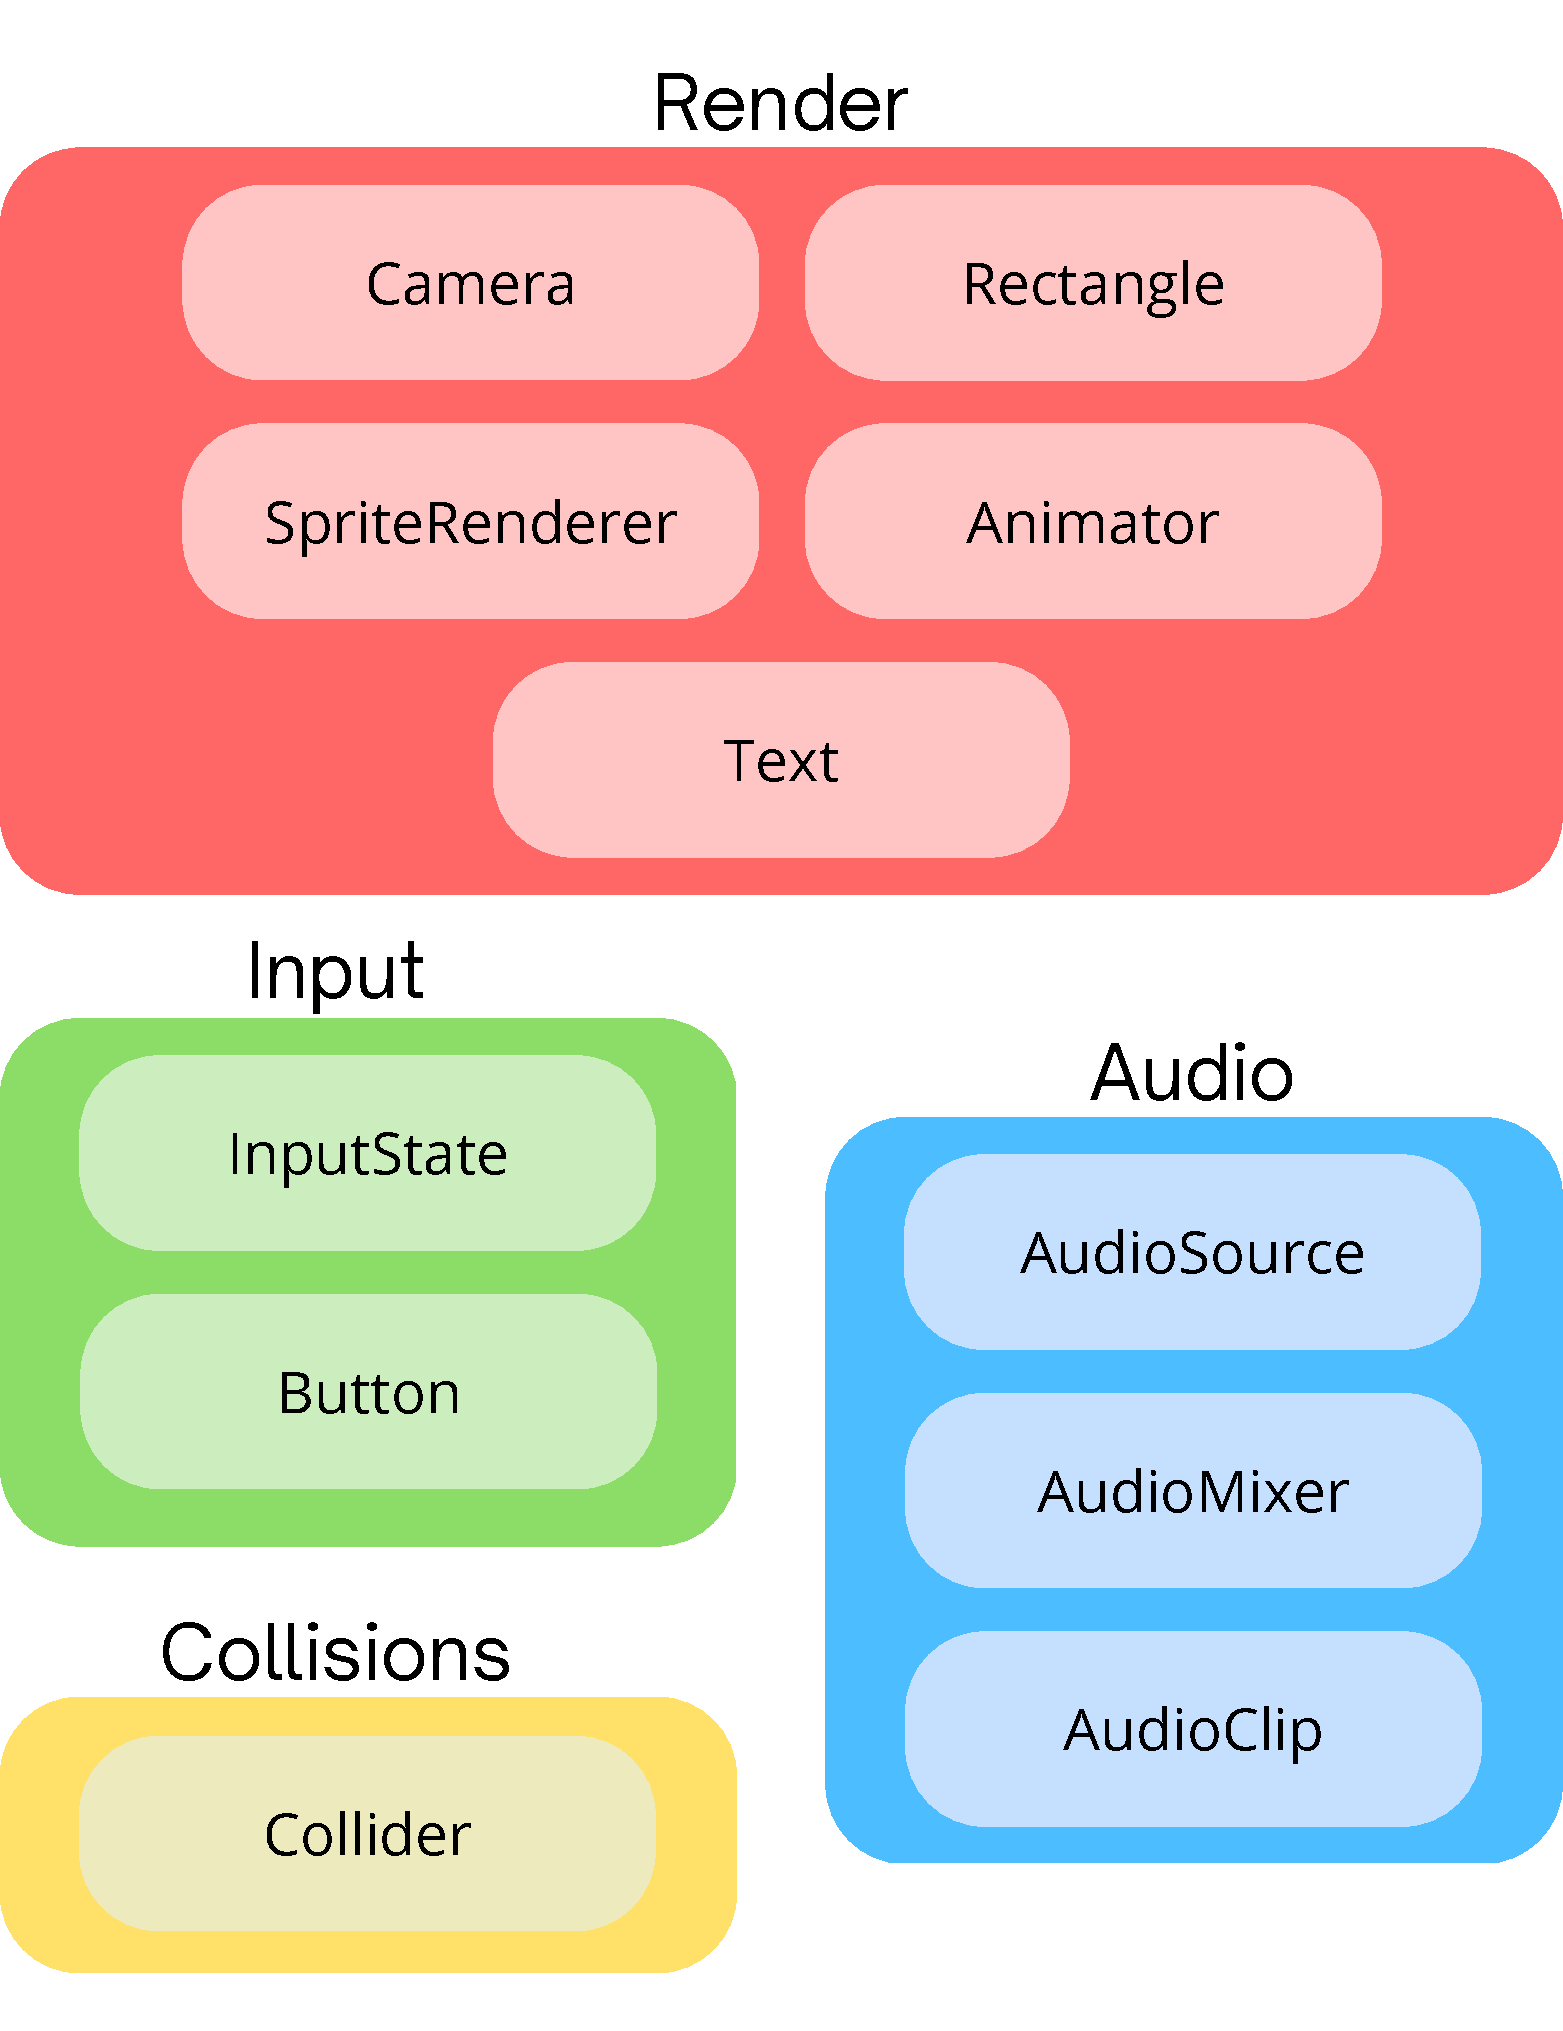
\includegraphics[height=0.85\textheight]{imgs/motor/ComponentesGenericos.pdf}
	\end{columns}
\end{frame}
\begin{frame}{Componentes específicos}
	\begin{columns}
		\column{0.5\textwidth}
			\begin{itemize}
				\item Sistema de diálogos.
				\item Sistema de movimiento.
				\item Sistema de mapas.
				\item Sistema de eventos.
			\end{itemize}
	 	\column{0.5\textwidth}
			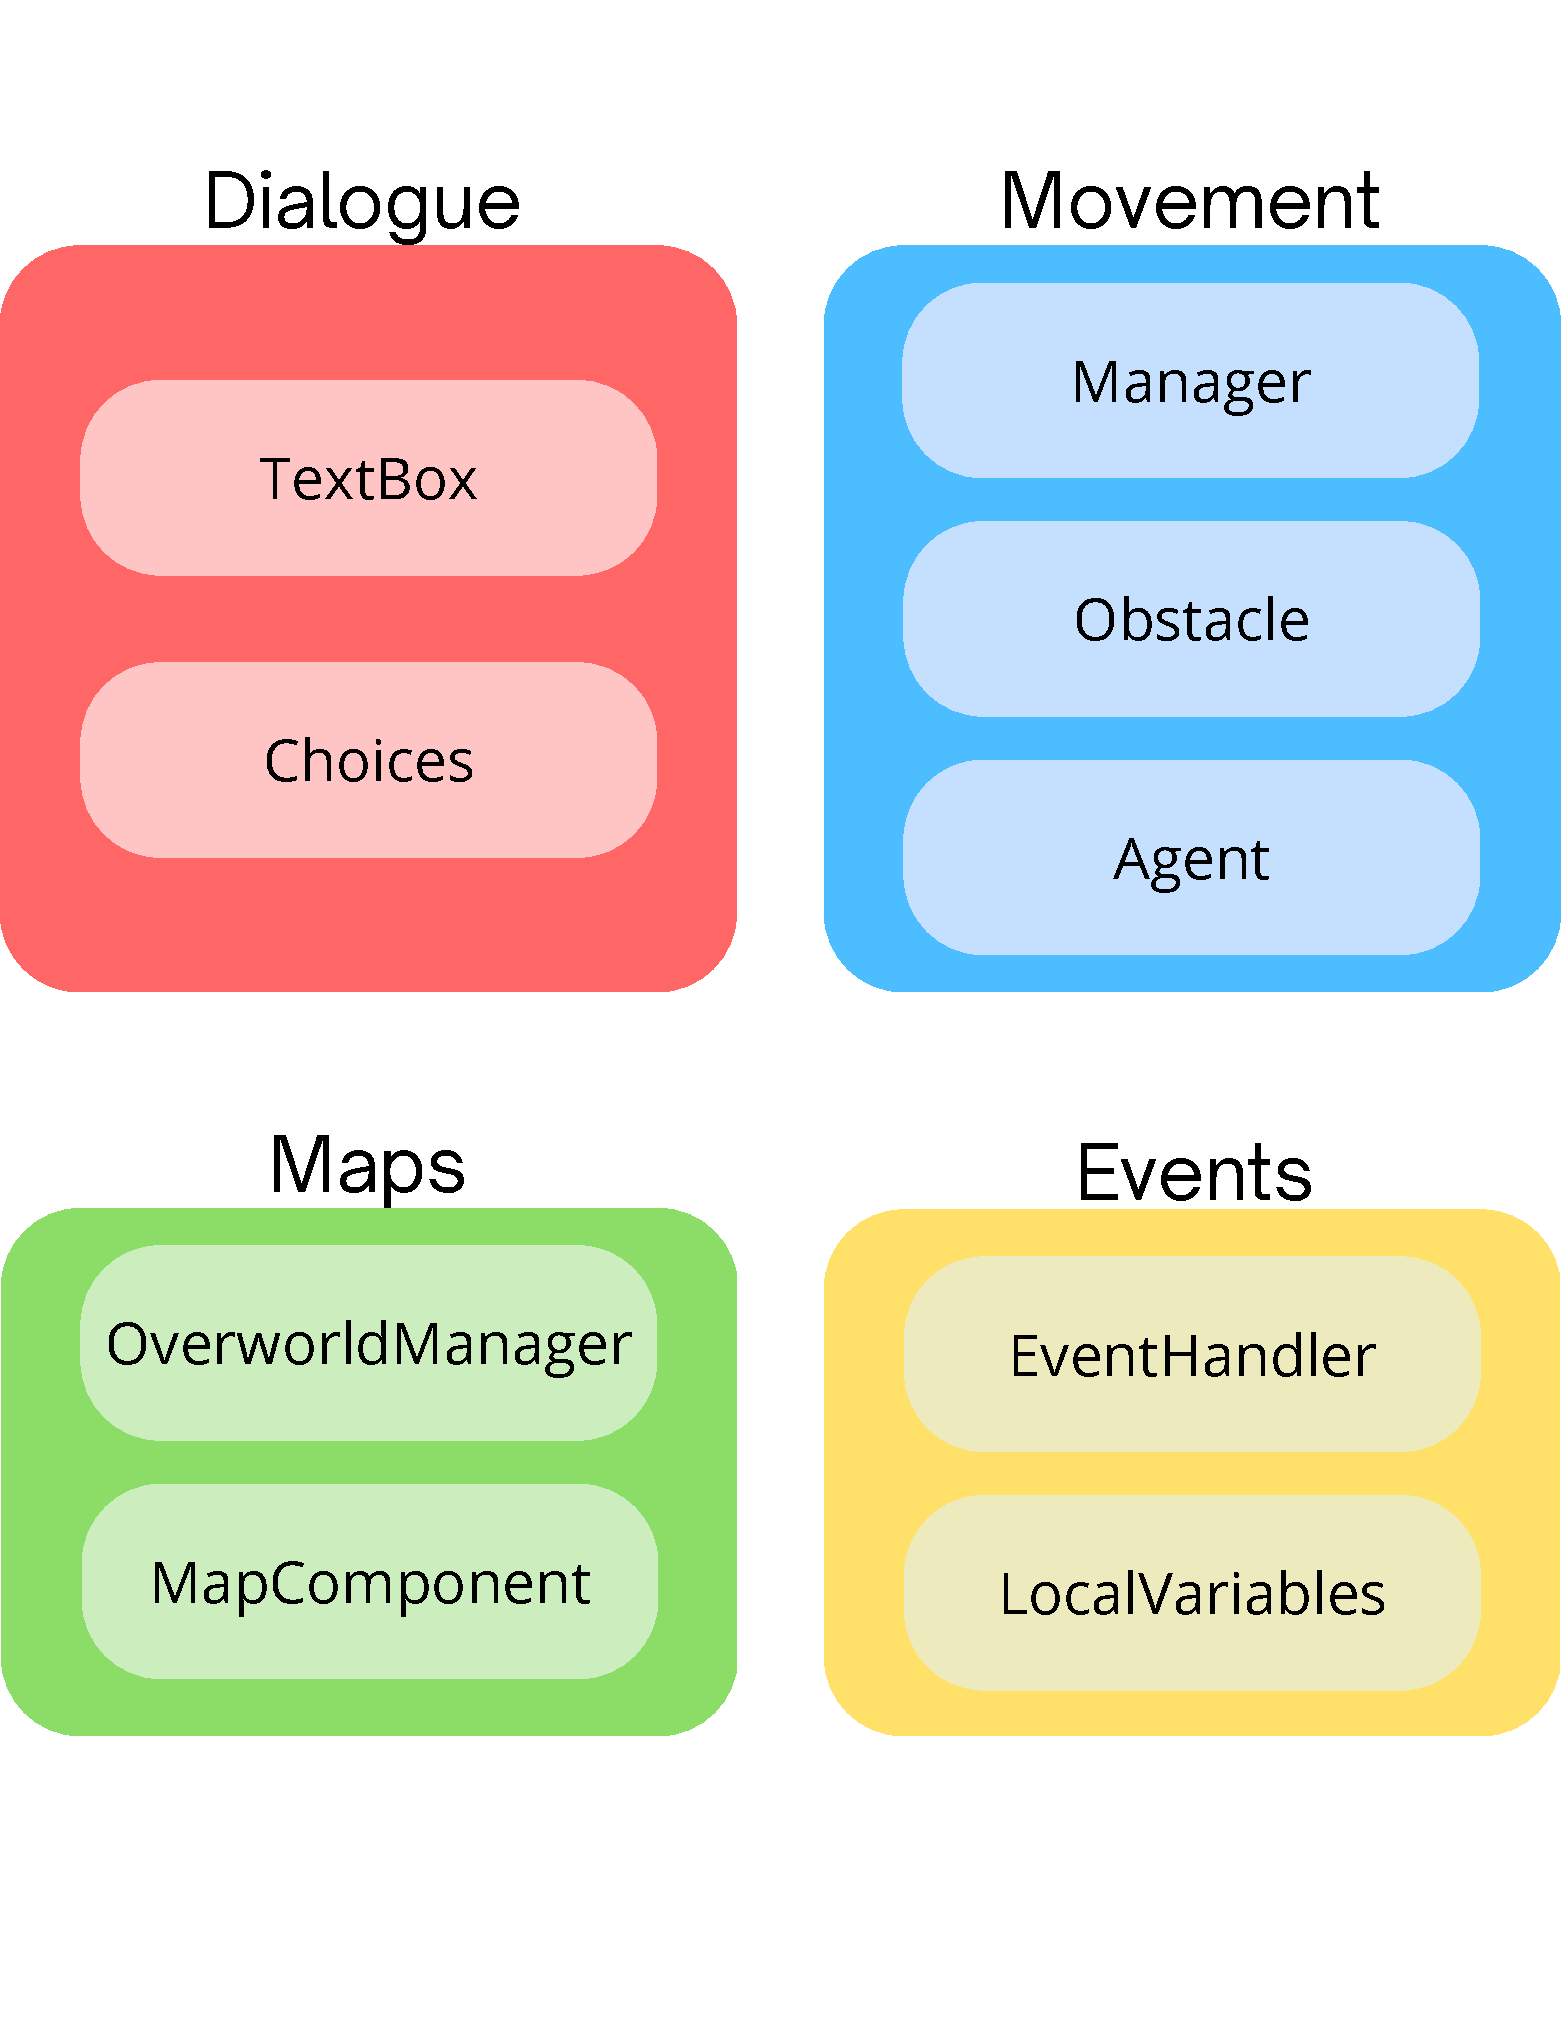
\includegraphics[height=0.85\textheight]{imgs/motor/ComponentesEspecificos.pdf}
	\end{columns}
\end{frame}
\begin{frame}{Eventos}
	\begin{columns}
		\column{0.5\textwidth}
			\begin{itemize}
				\item Condiciones.
				\item Comportamientos.
				\item Integración con el editor.
			\end{itemize}
	 	\column{0.5\textwidth}
 				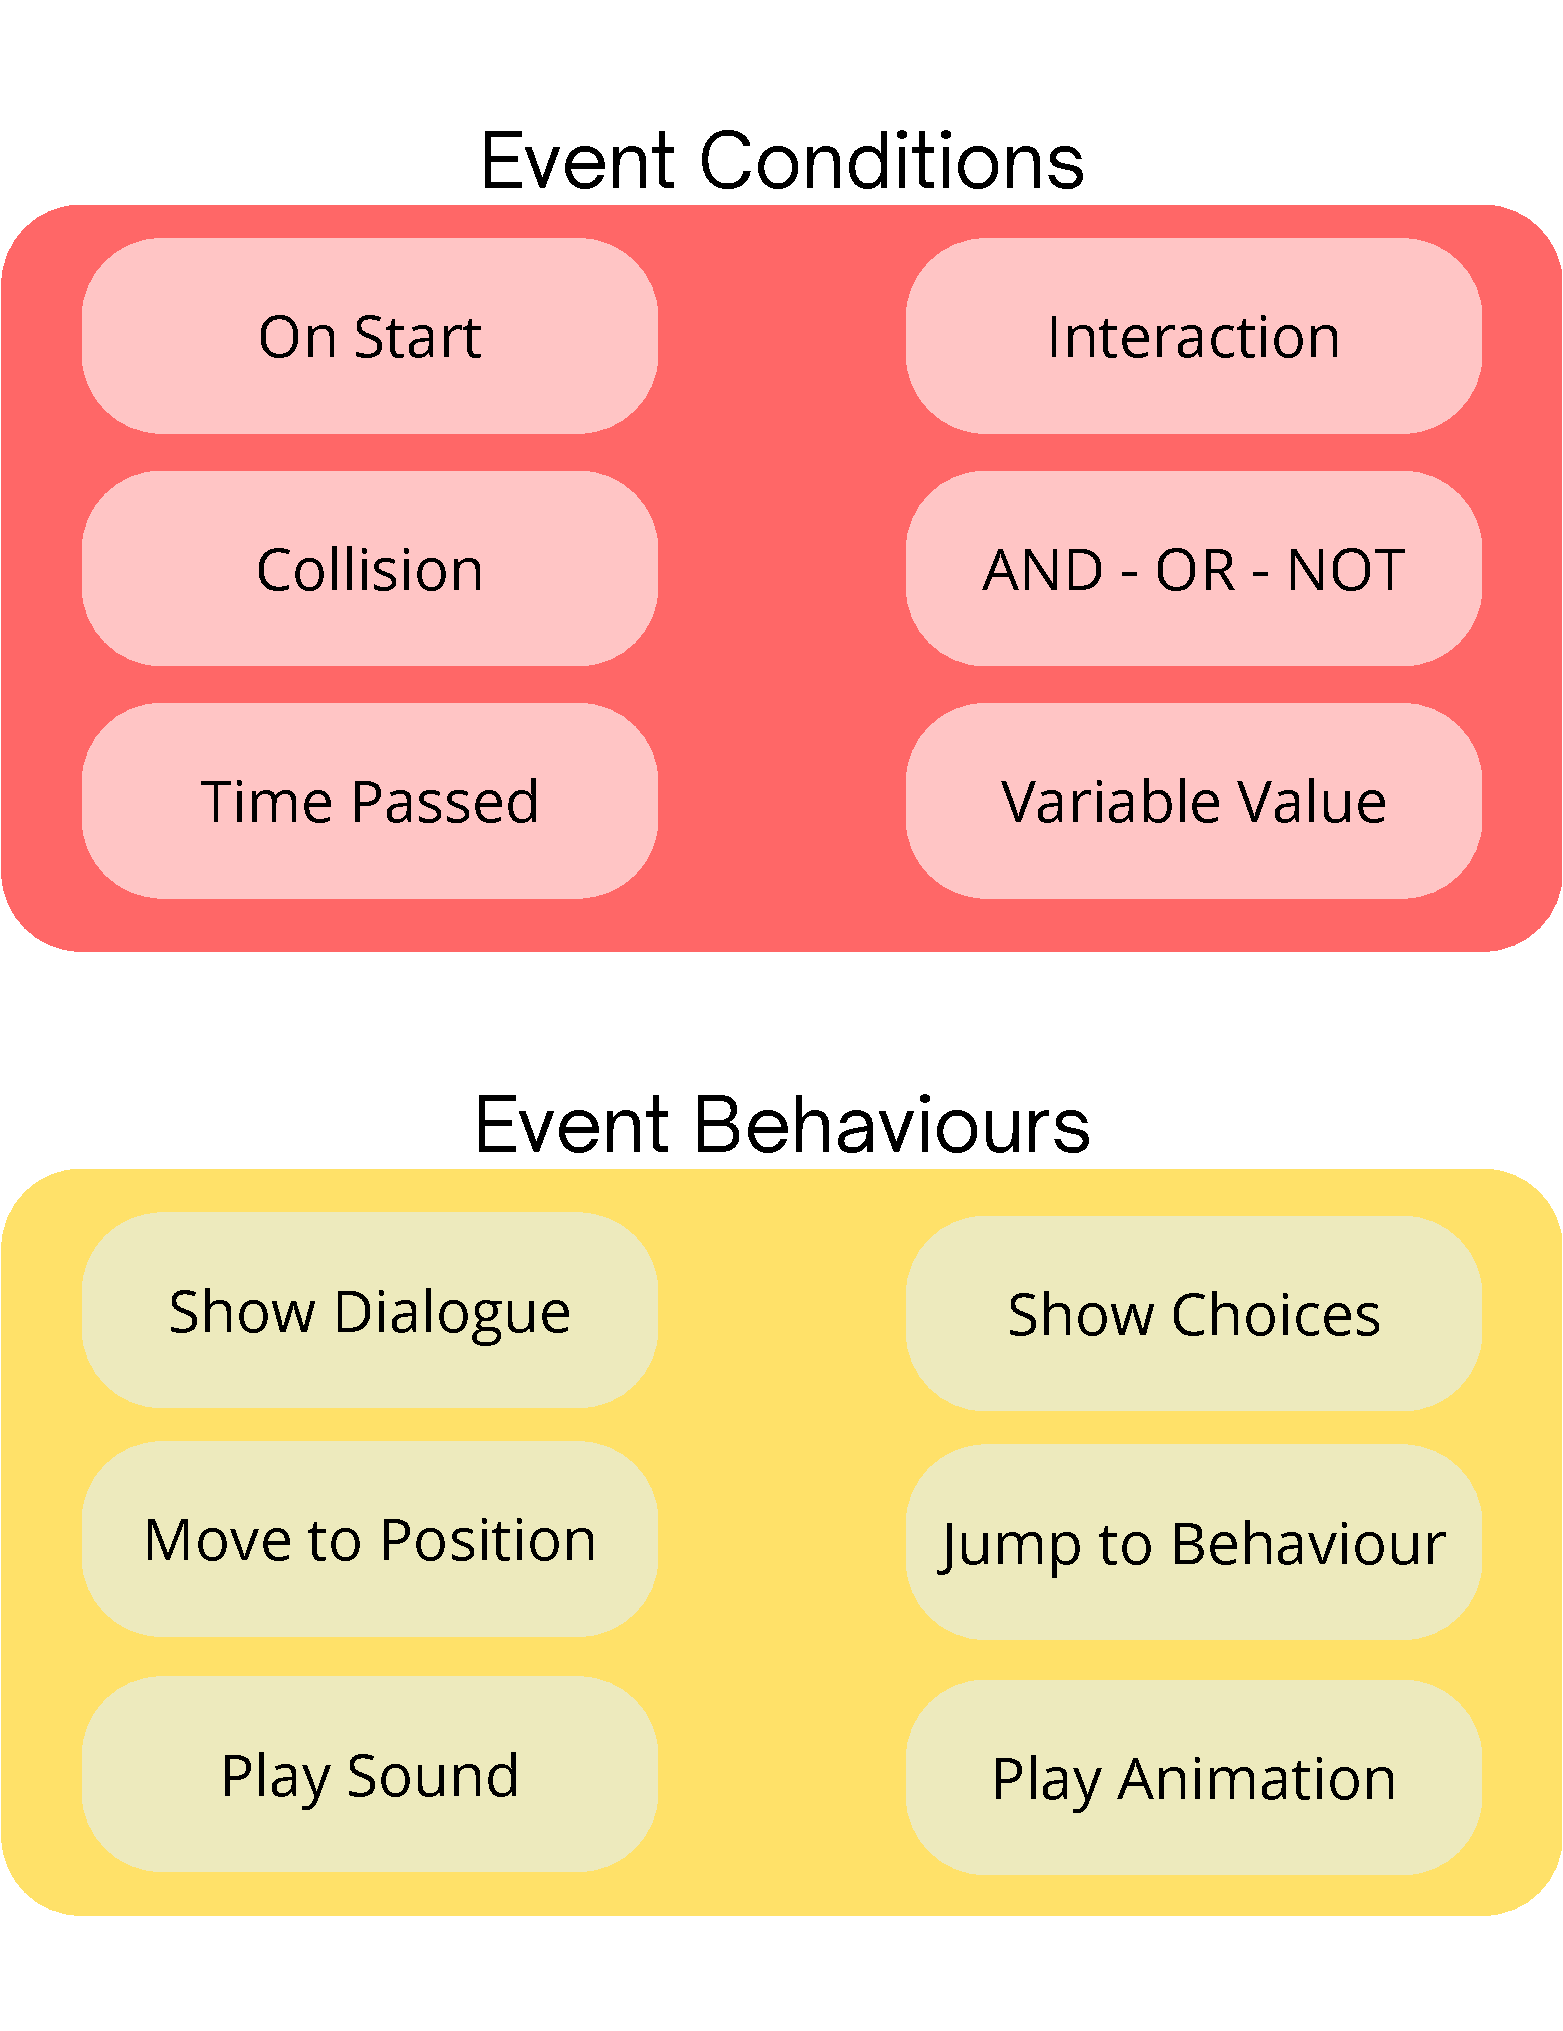
\includegraphics[height=0.85\textheight]{imgs/motor/Eventos.pdf}
	\end{columns}
\end{frame}
\section{Diseño del editor de \baker}
\begin{frame}{Editor de \baker}
	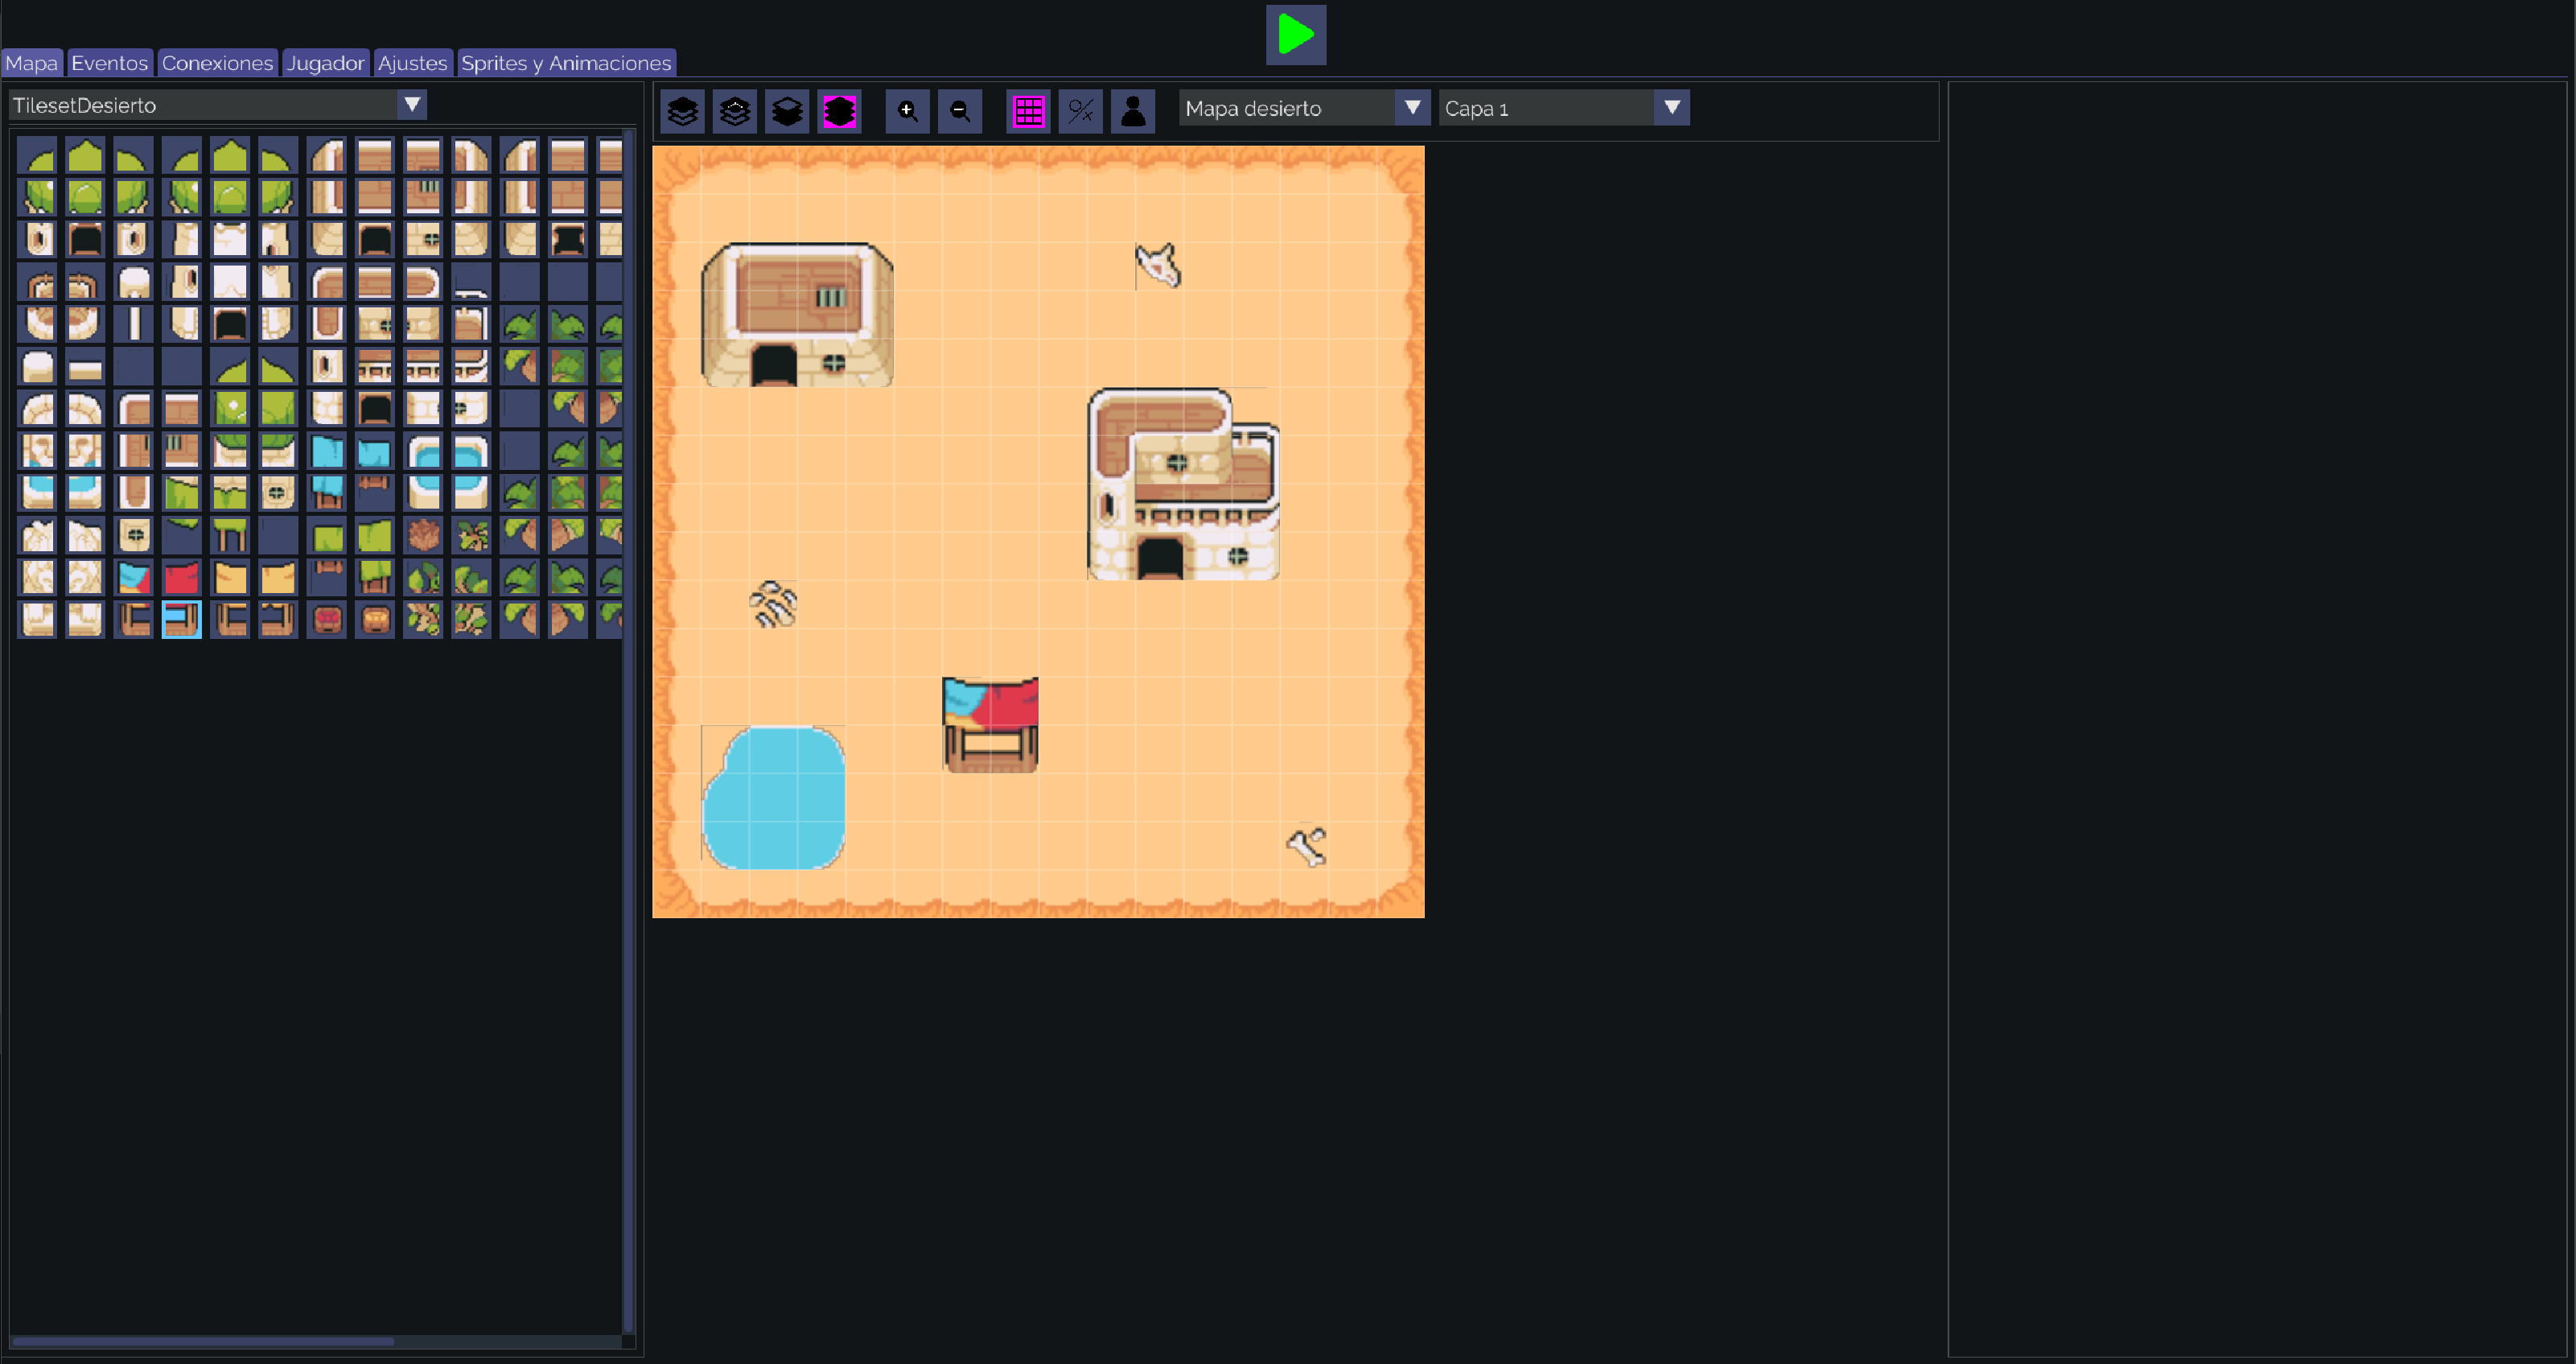
\includegraphics[width=\textwidth]{imgs/editor/editorMapas.pdf}
\end{frame}

\begin{frame}{Funcionalidades principales}
	\begin{columns}
		\column{0.4\textwidth}
			\begin{itemize}
				\item Edición de mapas de manera interactiva.
				\item Gestión de recursos gráficos, como \textit{sprites} o animaciones.
				\item Edición de eventos con condiciones y comportamientos personalizables.
				\item Carga y guardado de proyectos con persistencia completa.
			\end{itemize}
		\column{0.6\textwidth}
			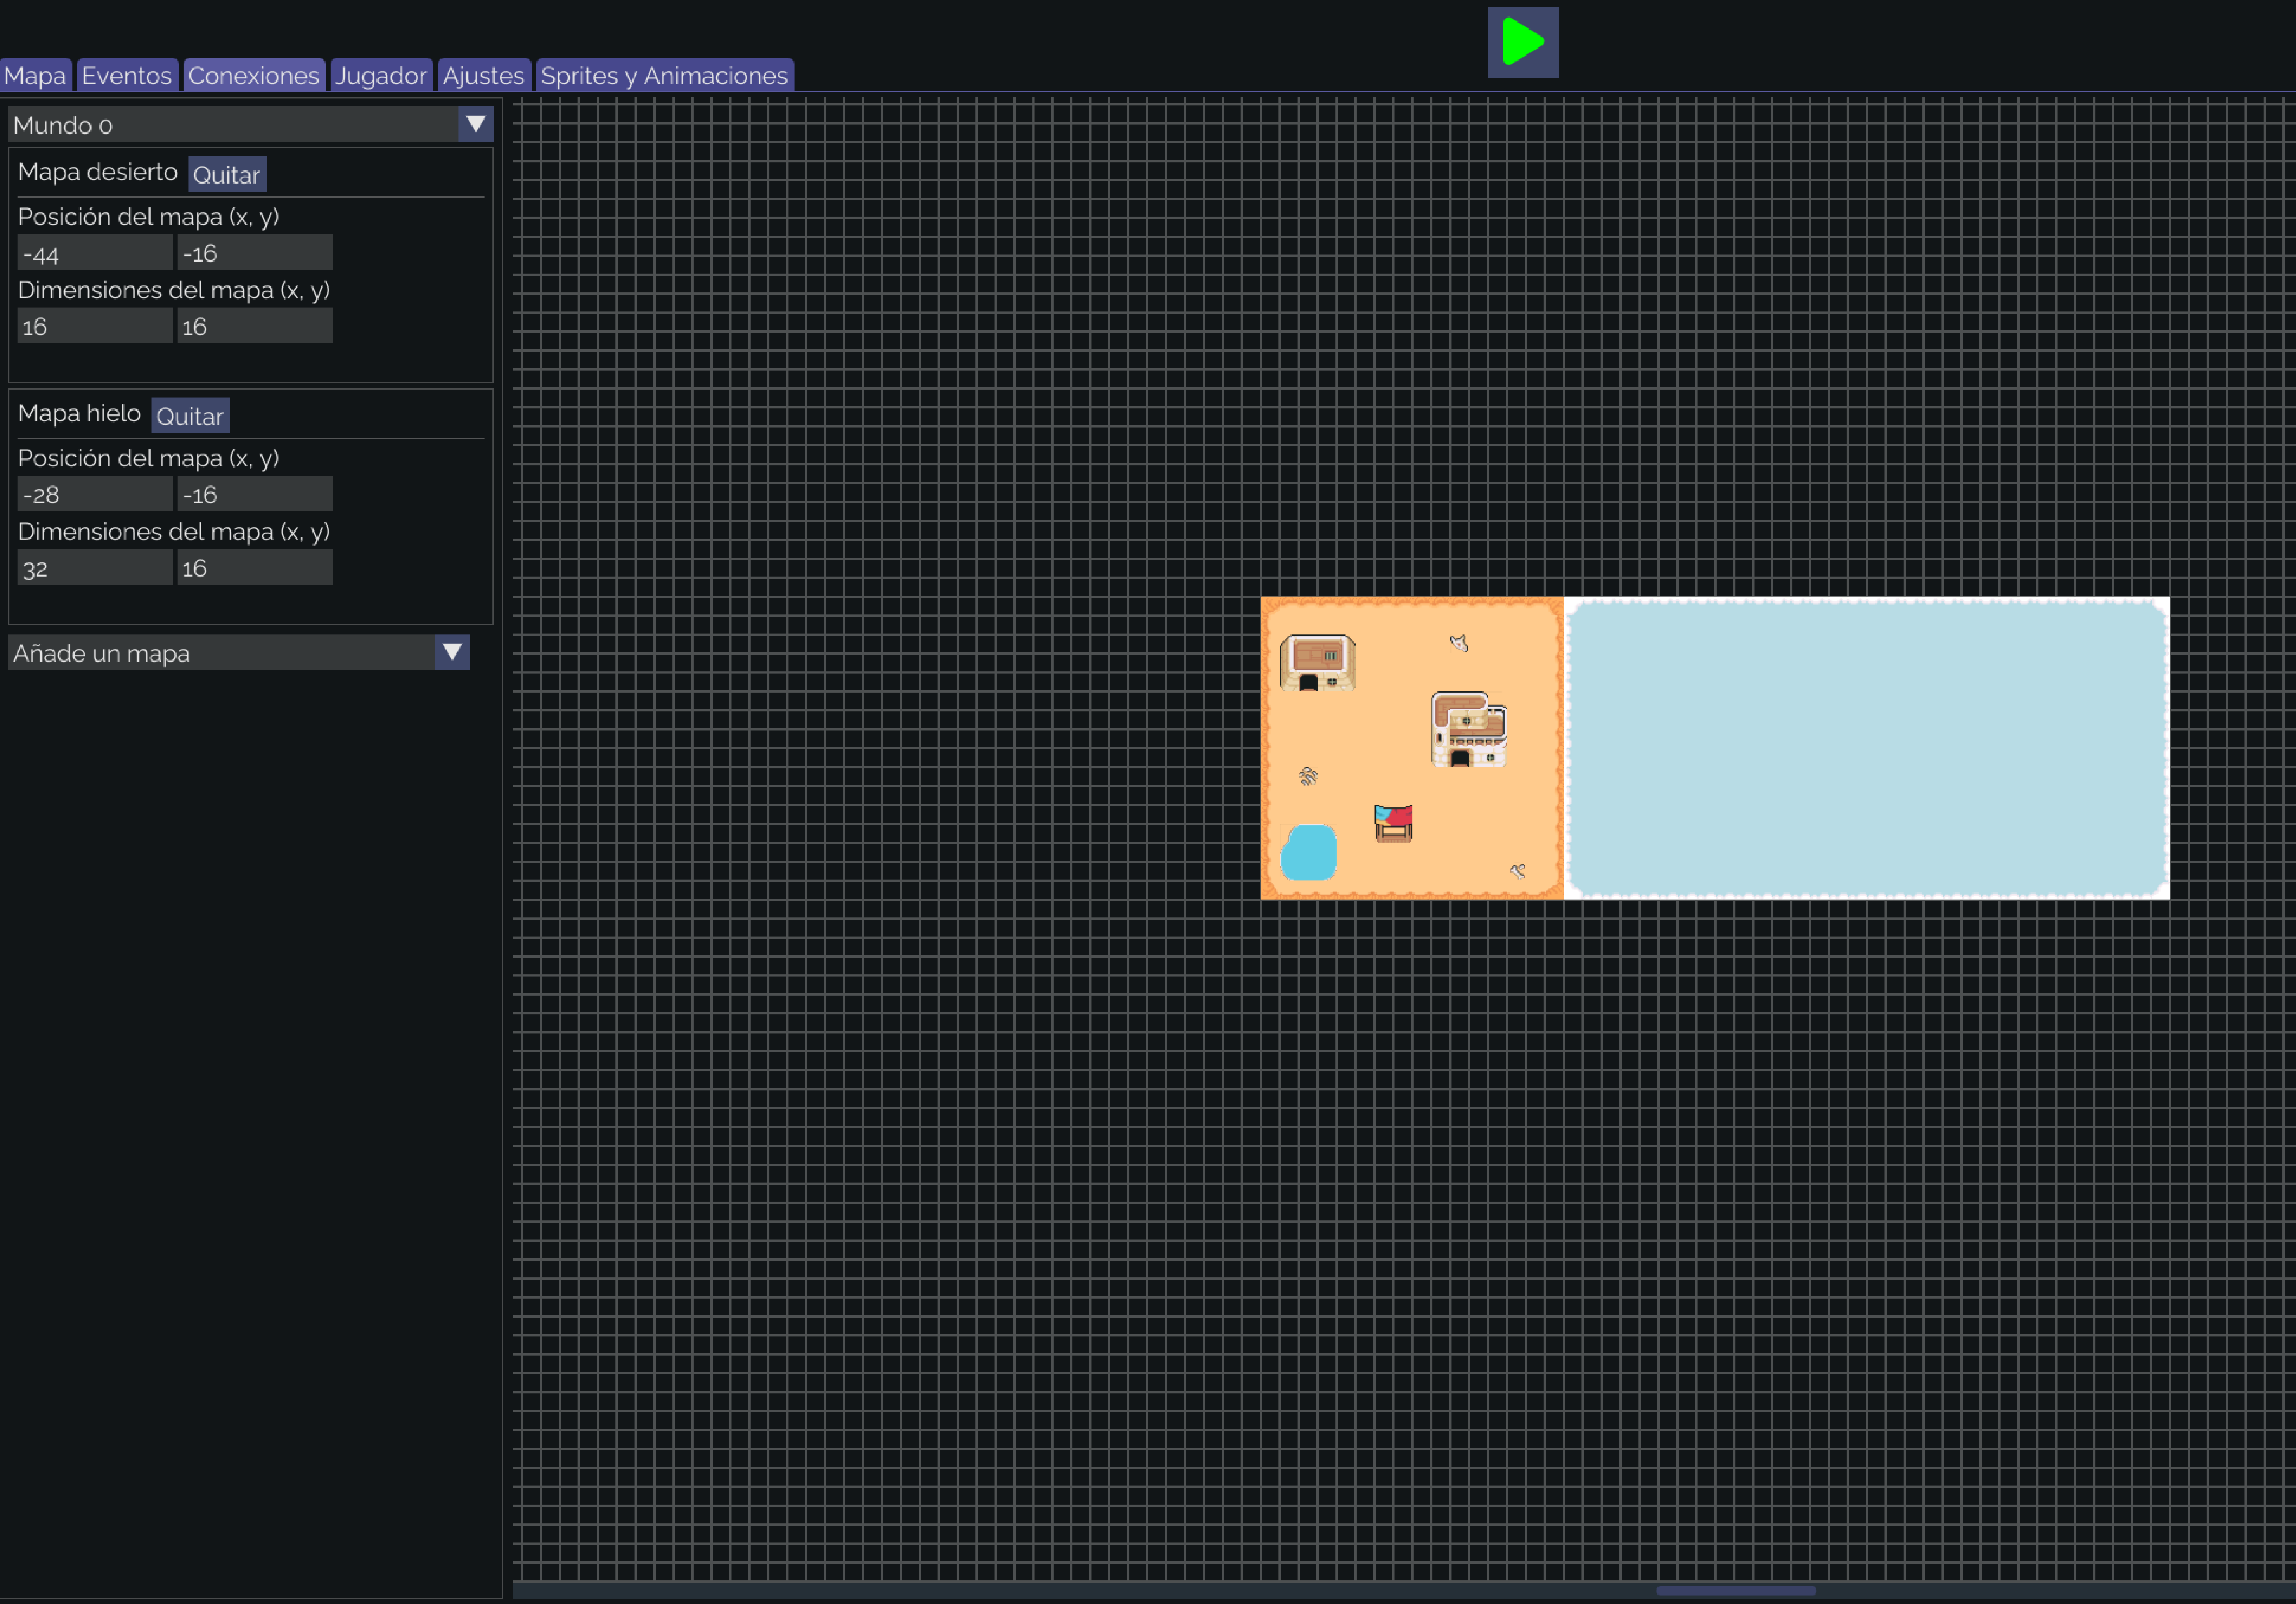
\includegraphics[width=\textwidth]{imgs/editor/conexiones.pdf}
	\end{columns}
\end{frame}

\begin{frame}{Interfaz y usabilidad}
	\begin{columns}
		 \column{0.4\textwidth}
		 	\begin{itemize}
		 		\item Interfaz basada en ventanas y pestañas: clara, modular y adaptable.
		 		\item Pensada para usuarios novatos.
		 		\item Pestañas dependiendo de su función: editor de mapas, de eventos, de recursos\ldots
		 		\item Soporte de elementos visuales como \textit{tooltips} o mensajes de error.
		 	\end{itemize}
		 \column{0.6\textwidth}
		 	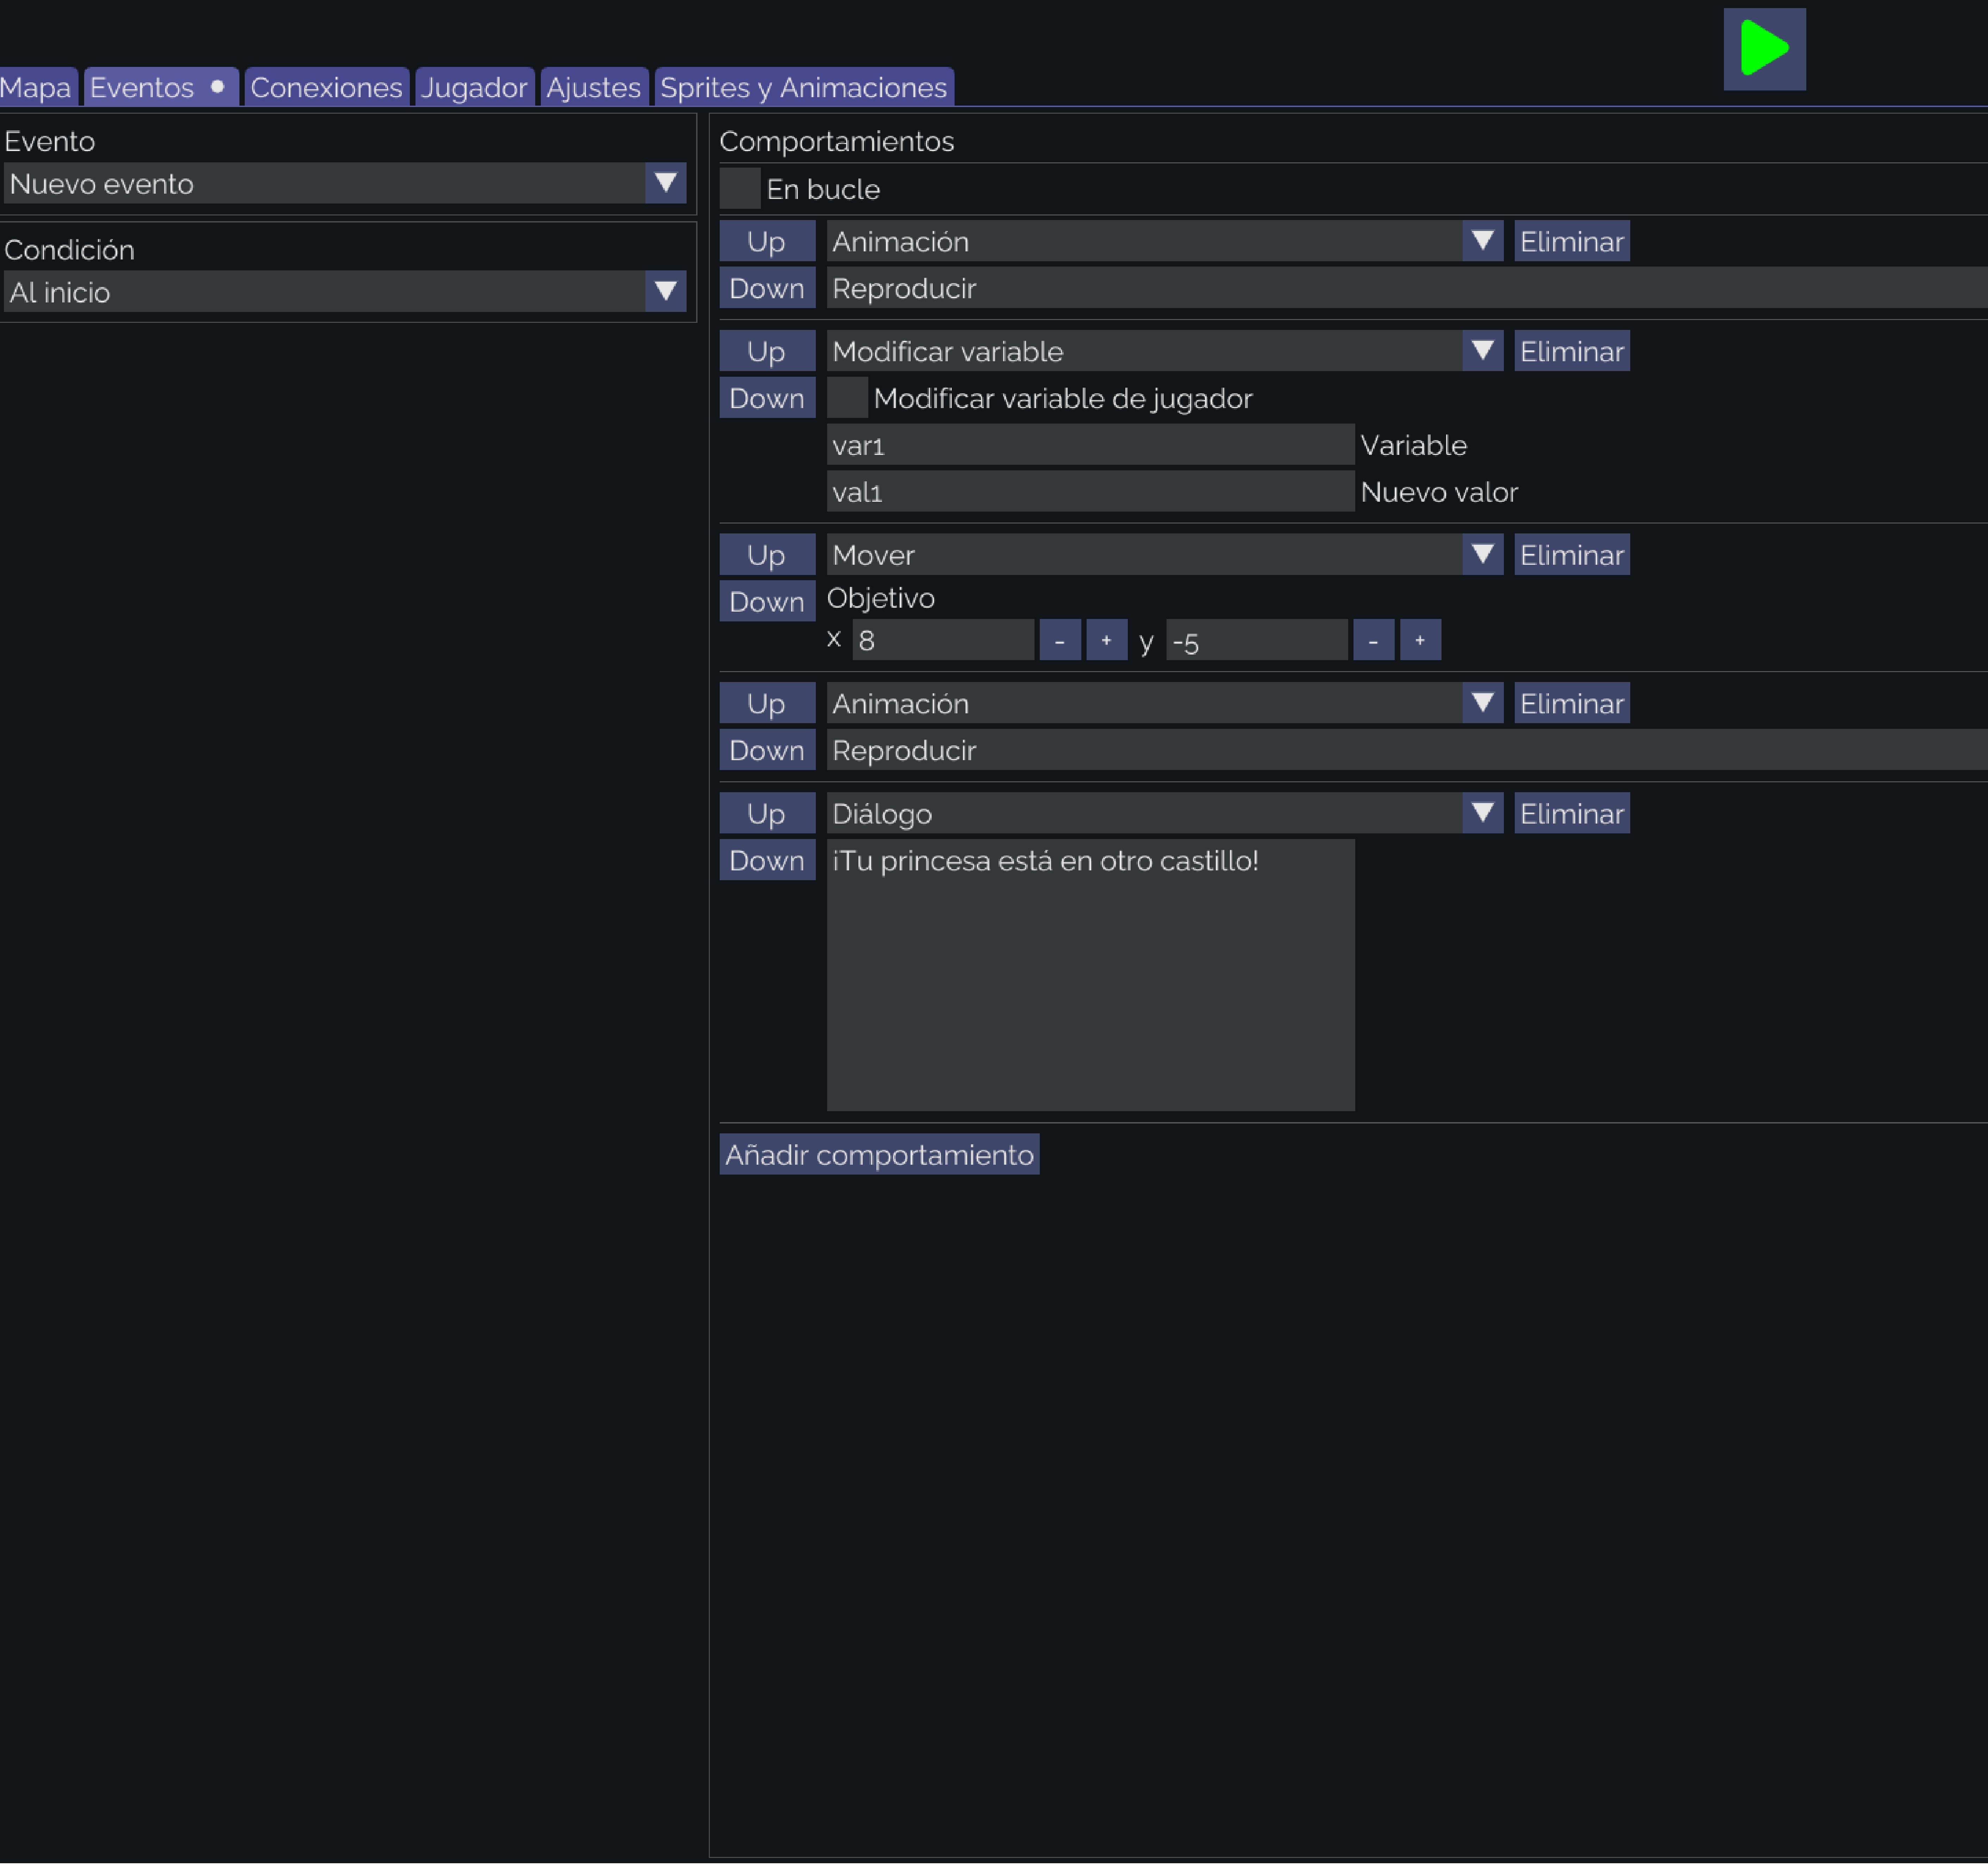
\includegraphics[width=0.9\textwidth]{imgs/editor/eventos.pdf}
	\end{columns}
\end{frame}

\begin{frame}{\textit{Build} multiplataforma al motor}
	\begin{columns}
		 \column{0.4\textwidth}
		 	\begin{itemize}
		 		\item Se generan ejecutables para Windows, MacOS, Linux y Android.
		 		\item No requiere de recompilación manual ni de pasos adicionales.
		 		\item El editor \comillas{traduce} sus datos a la sintaxis esperada por el motor.
		 	\end{itemize}
		 \column{0.6\textwidth}
		 	\begin{center}
		 	\scalebox{0.6}{
		 	\begin{tikzpicture}[node distance=1.5cm and 2cm]
		 		\node (start) [startstop] {Usuario diseña el juego en el editor};
		 		\node (data) [process, below=of start] {Datos del proyecto};
				\node (convert) [process, below=of data] {Serialización y empaquetado};
				\node (build) [process, below=of convert] {Generación del ejecutable};
				\node (win) [io, below left=1.5cm and 2.5cm of build] {Windows};
				\node (mac) [io, below left=1.5cm and -1.0cm of build] {MacOS};
				\node (linux) [io, below right=1.5cm and -1.0cm of build] {Linux};
				\node (andr) [io, below right=1.5cm and 2.5cm of build] {Android};
				
				\draw [arrow] (start) -- (data);
				\draw [arrow] (data) -- (convert);
				\draw [arrow] (convert) -- (build);
				\draw [arrow] (build) -- (win);
				\draw [arrow] (build) -- (mac);
				\draw [arrow] (build) -- (linux);
				\draw [arrow] (build) -- (andr);
		 	\end{tikzpicture}
		 	}
		 	\end{center}
	\end{columns}
\end{frame}


\section{Pruebas con usuarios}
\begin{frame}{Objetivos de las pruebas}
	\begin{itemize}
		\item ¿Entienden los usuarios cómo funcionan los sistemas?
		\item ¿Son capaces de aprovecharlos de forma creativa?
	\end{itemize}
\end{frame}
\begin{frame}{Metodología}
\begin{columns}
	\column{0.4\textwidth}
	\begin{itemize}
		\item Pruebas individuales supervisadas.
		\item Guía explicativa.
		\item Usuarios con distinto nivel.
	\end{itemize}
	\column{0.6\textwidth}
	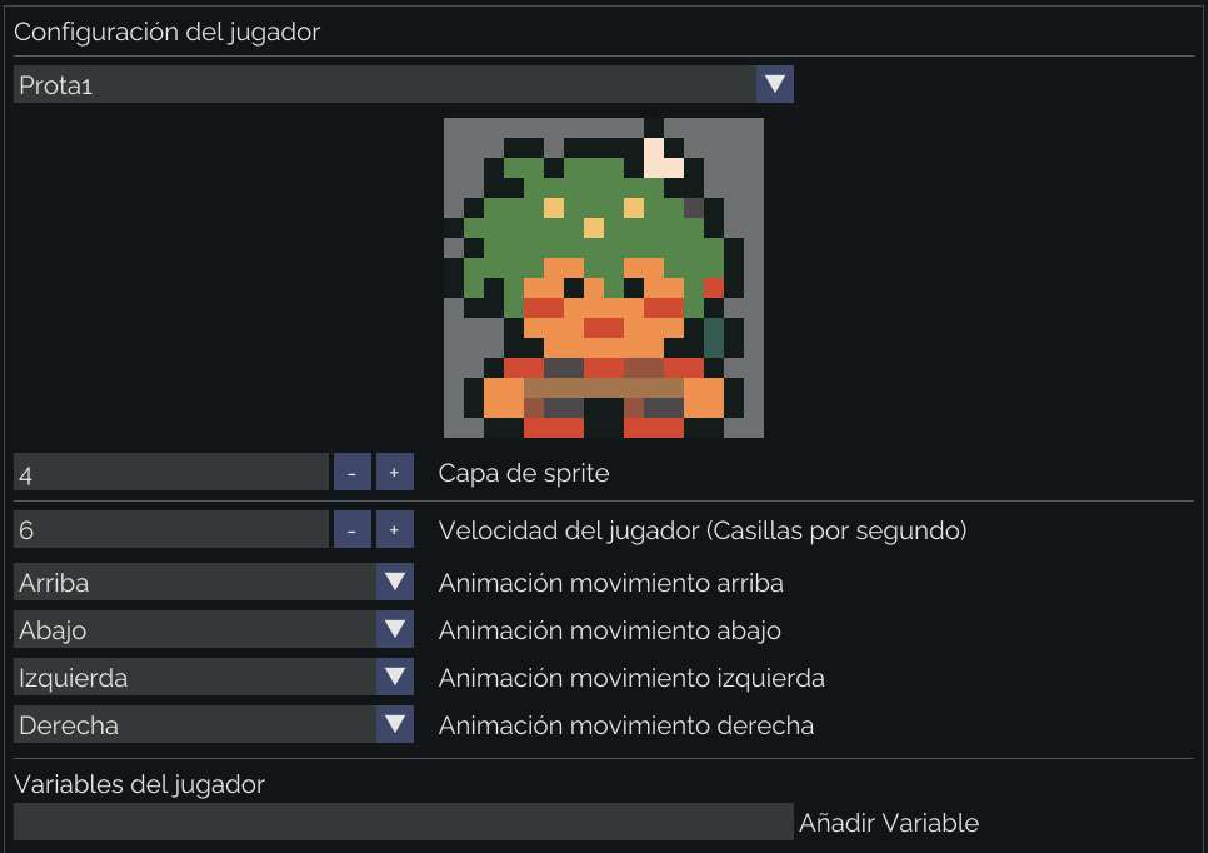
\includegraphics[width=\textwidth]{imgs/pruebas/metodologia.pdf}
\end{columns}
\end{frame}
\begin{frame}{Resultados}
\begin{columns}
	\column{0.4\textwidth}
	\begin{itemize}
		\item Los sistemas se entienden.
		\item Permiten la creatividad.
		\item A pesar de esto pueden ser limitados y toscos.
	\end{itemize}
	\column{0.6\textwidth}
	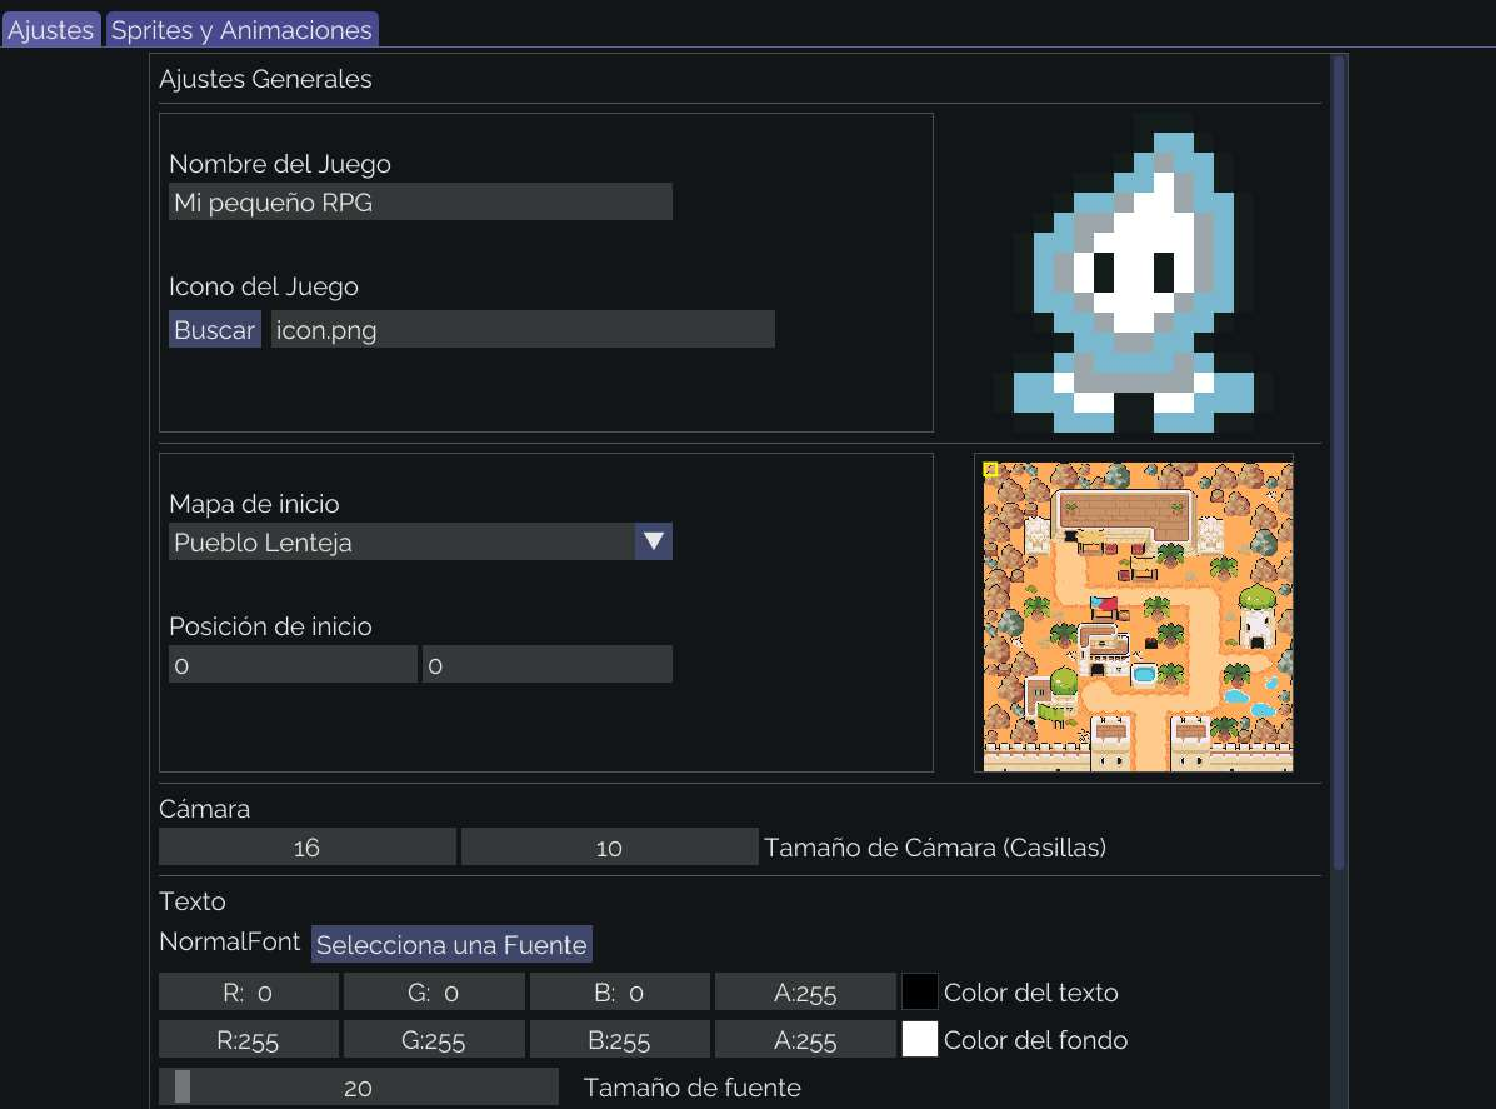
\includegraphics[width=\textwidth]{imgs/pruebas/resultados.pdf}
\end{columns}
\end{frame}

\section{Conclusiones}
\begin{frame}{Conclusiones y trabajo futuro}
\begin{columns}
	\column{0.4\textwidth}
	\begin{itemize}
		\item Creación accesible de RPG.
		\item Desarrollo de juegos multiplataforma.
		\item Futuros sistemas de combate e inventario.
	\end{itemize}
	\column{0.6\textwidth}
	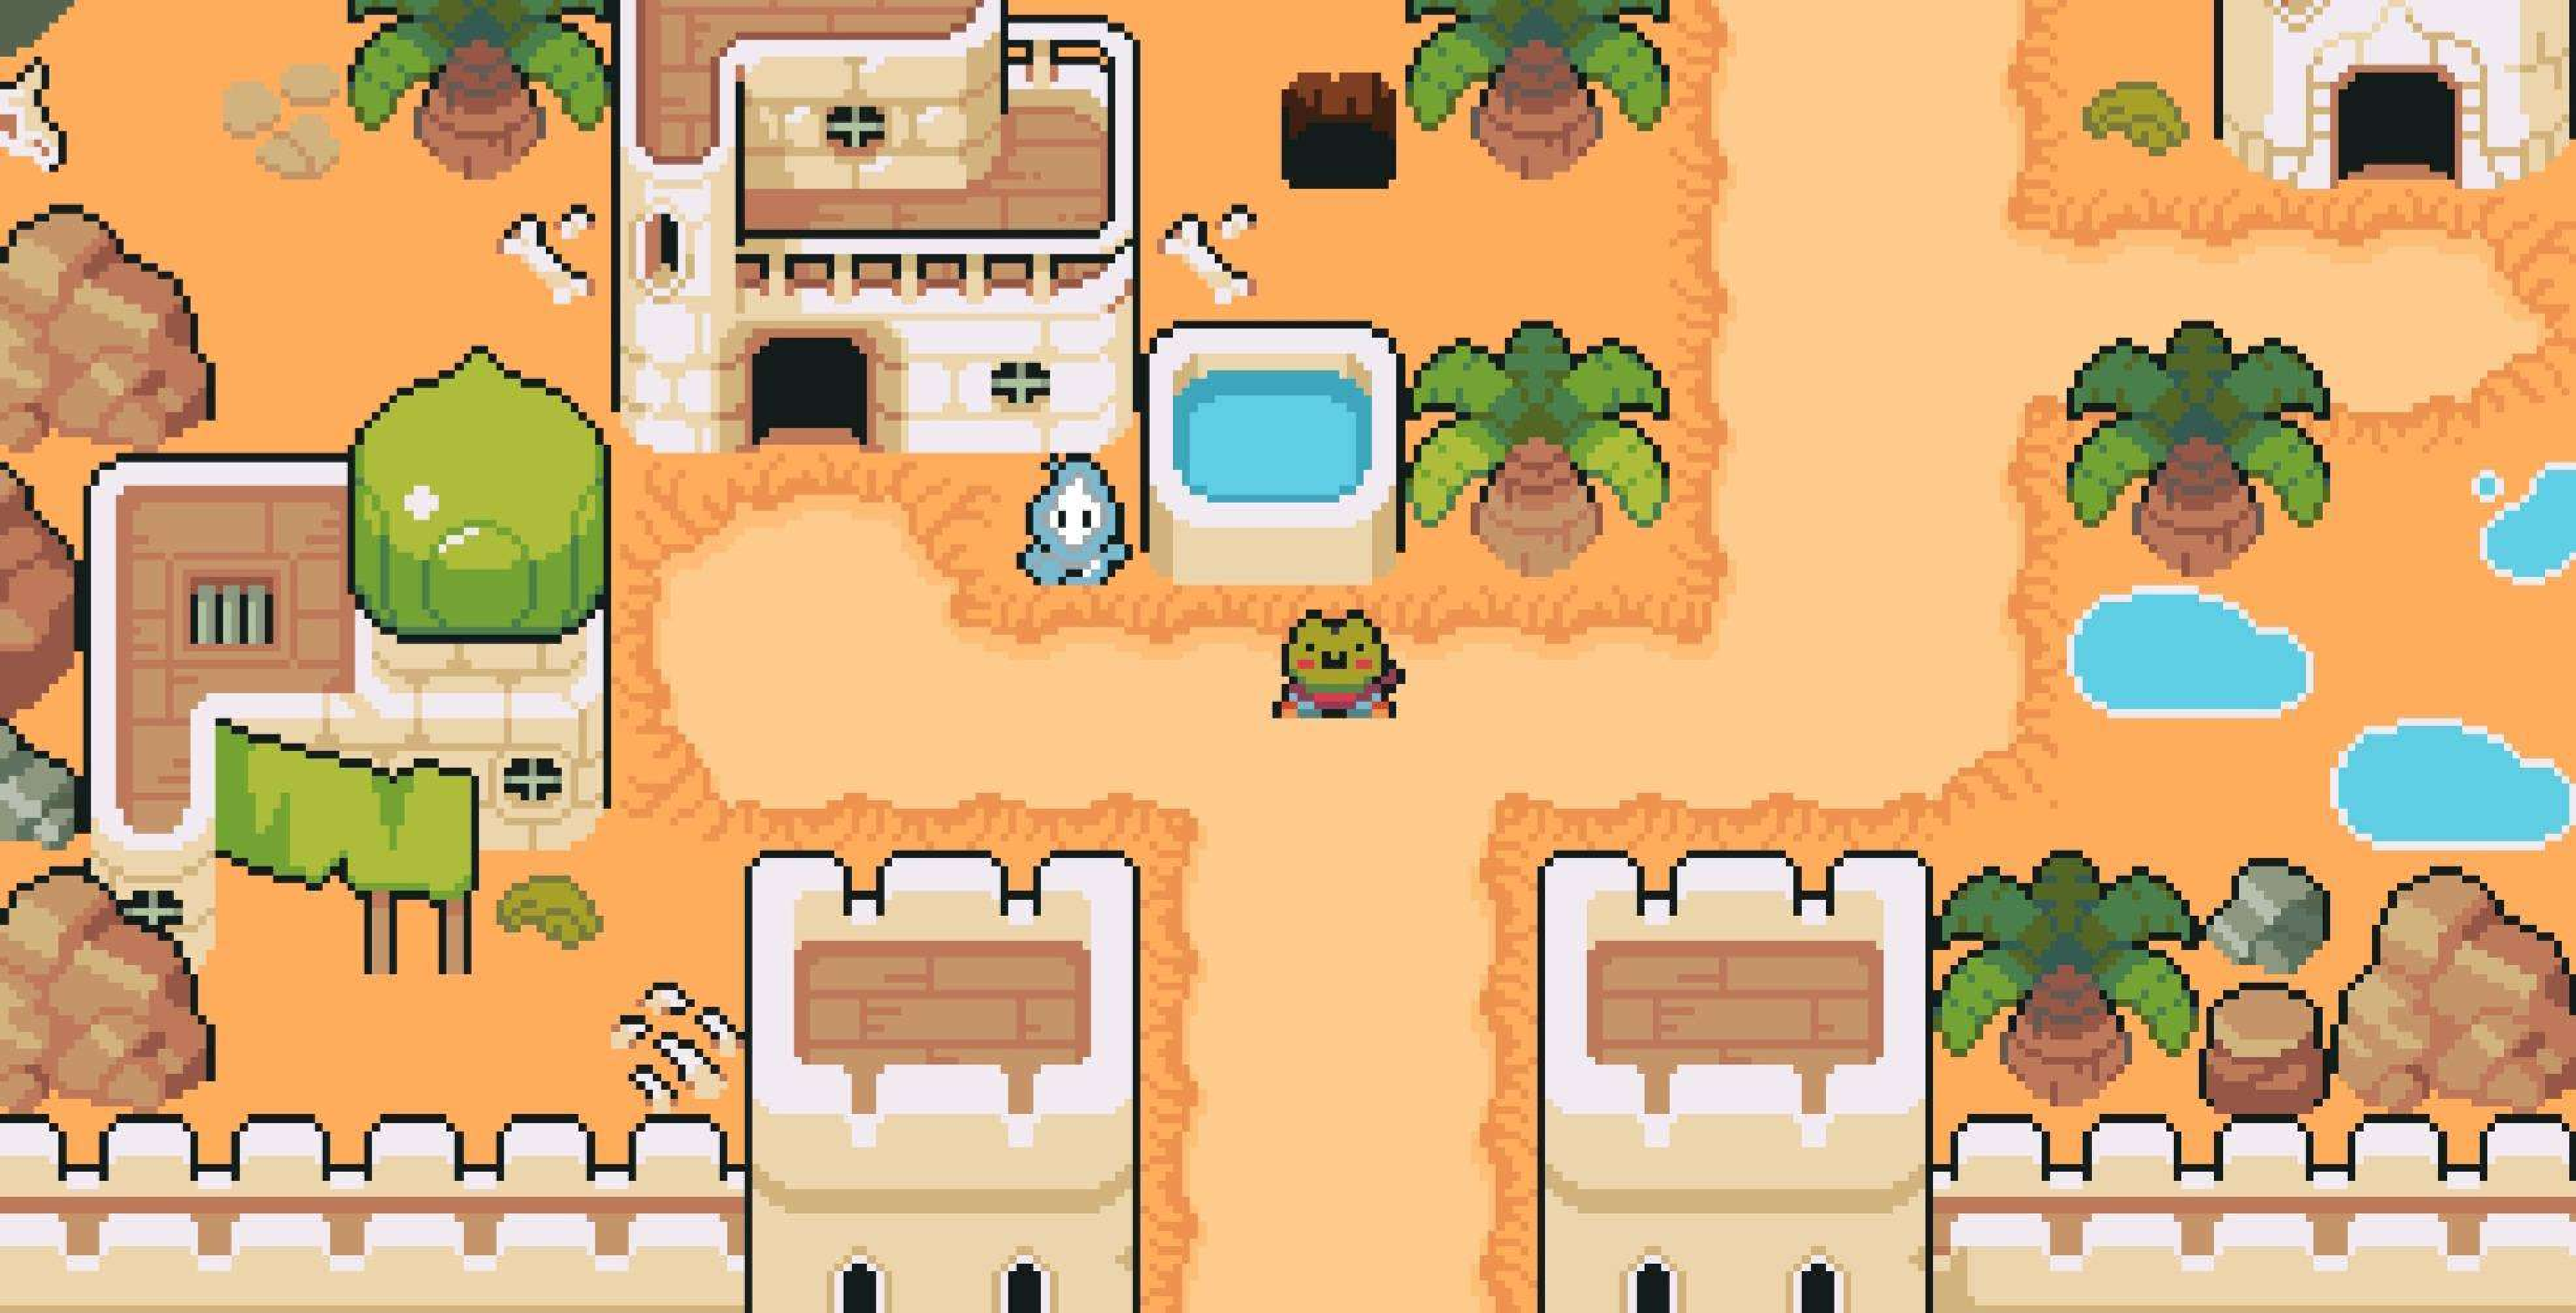
\includegraphics[width=\textwidth]{imgs/conclusiones/conclusiones.pdf}
\end{columns}
\end{frame}


\title[2D video game engine and editor focused on RPG game development]{Motor y editor de videojuegos en 2D enfocado al desarrollo de juegos RPG}
\author[Miguel Curros, Alejandro González and Alejandro Massó]{Miguel Curros García\\ Alejandro González Sánchez\\ Alejandro Massó Martínez}

\section{Contributions}
\begin{frame}{Miguel Curros García}
	\begin{itemize}
		\item \baker{}'s engine design.
		\item Engine low level development.
		\item Engine gameplay development.
		\item Editor resources' persistance.
		\item Editor's events' interface
		\item Editor's events' build.
	\end{itemize}
\end{frame}

\begin{frame}{Alejandro González Sánchez}
	\begin{itemize}
		\item Technical proof of concept
		\item \baker{}'s engine design.
		\item Engine low level development.
		\item Engine gameplay development.
		\item \baker{}'s Editor's interface development.
		\item Editor's building process.
	\end{itemize}
\end{frame}

\begin{frame}{Alejandro Massó Martínez}
	\begin{itemize}
		\item Research on general and specific RPG editors.
		\item \baker{}'s editor design.
		\item Project's toolchain development.
		\item \baker{}'s editor development.
		\item Report writing.
	\end{itemize}
\end{frame}

\begin{frame}{¿Preguntas?}
	\begin{center}
		
\includegraphics[width=0.4\textwidth]{imgs/cmn/preguntas.pdf}
	\end{center}
\end{frame}

\end{document}